% !TEX root = template.tex

\section{Processing Pipeline}
\label{sec:processing_architecture}

\begin{figure*}[h]
	\centering
	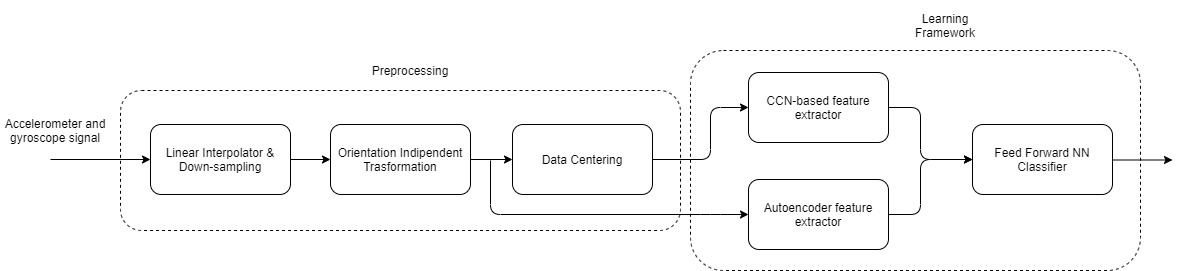
\includegraphics[width=1\textwidth]{images/processing_pipeline.jpg}
	\caption{Processing pipeline}
\end{figure*}

Spiegare ad alto livello tutta la pipeline di preprocessing adottata, i vari blocchi a che cosa servono!

\section{Signals and Features}
\label{sec:model}

In questo caso si va nel dettaglio della parte di preprocessing (parte trattegiata nel mio schema come preprocessing)

Parlare del dataset, come sono stati processati i dati (interpolazione lineare), parlare della time-window applicata di 2,5s, e parlare del rotational indipendent trasform per ruorare nuovamente i dati. L'applicazione del centering per la sola rete CNN e l'estrazione delle basic feature per risimulare il lavoro fatto in \cite{ignatov2018real}.

\subsection{Dataset \& Meausurement Setup}
Parlare di come abbiamo splittato il dataset, quindi escludendo gli utenti a e b per fare in modo di testare le performance cambiando compltamente utente.

Introduzione e spiegazione del dataset eterogeneo, preso da: riportare link.

Accenare dell'acquisizione di un nostro dataset alla stessa maniera, a 100 HZ in varie posizioni per testare poi anche tutto il dataset!

\subsection{Signal preprocessing}

\begin{itemize}
	\item interpolazione lineare / downsampling
	\item rotational invariant citare tutti i paper e come funziona
	\item centering
\end{itemize}

\subsection{Feature vector}
\begin{itemize}
	\item window strategy
	\item basic feature extraction
	\item autoencoder feature extraction
\end{itemize}

\section{Learning Framework}
\label{sec:learning_framework}

\begin{figure*}[h]
	\centering
	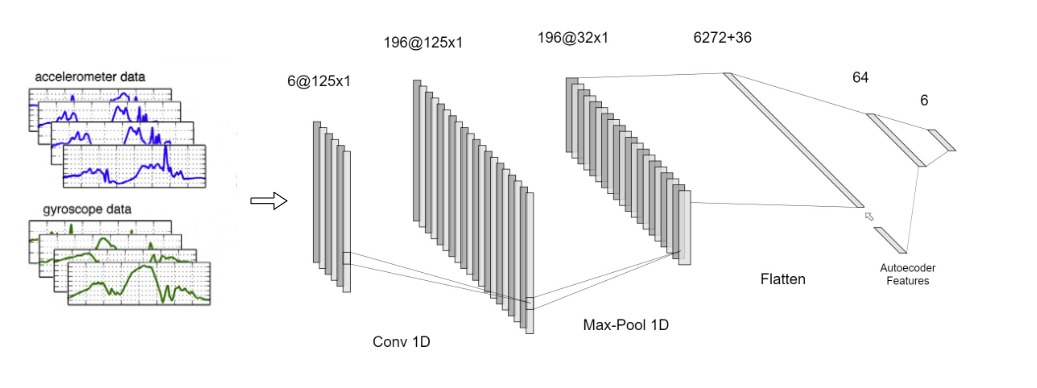
\includegraphics[width=1\textwidth]{images/full_architecture.jpg}
	\caption{Learning Framework}
\end{figure*}

Desctivere qui invece la parte tratteggiata come learning framework

Descivere prima l'autoencoder, come è stato costruito e come viene allenato. TODO luca

Passare alla decrizione della mia archittetura, come sono stai selezionati gli iper-parametri, ecc ecc.

